\documentclass{beamer}

\usepackage{stacks} % custom commands for typesetting stacks

\usepackage{listings,bold-extra}
\lstset{basicstyle=\ttfamily,
        mathescape=true,
        keepspaces=false,
        morekeywords={:=,+,-,*,/,goto,if,<,<=,>,>=,=}}
\usepackage{tikz}
\usetikzlibrary{shapes.misc}

\usepackage{../lib/minted}
\usemintedstyle{bw}
\newminted{factor}{gobble=0,frame=none}
\newmint{factor}{}

\usepackage{graphicx}
\newcommand{\whenNewer}[3]{%
  \ifnum\pdfstrcmp{\pdffilemoddate{#1}}%
  {\pdffilemoddate{#2}}>0%
  {\immediate\write18{#3}}\fi%
}
\newcommand{\includesvg}[2][]{%
  \whenNewer{#2.svg}{#2.pdf}%
    {inkscape -z -D --file=#2.svg --export-pdf=#2.pdf}%
  \includegraphics[#1]{#2.pdf}%
}

\newcommand{\vn}[1]{\ensuremath{\langle\texttt{#1}\rangle}}
\newcommand{\vreg}[1]{\texttt{#1}}

\mode<presentation>{
  \usetheme{CambridgeUS}
  \useoutertheme{infolines}
  \setbeamertemplate{navigation symbols}{}
  %\AtBeginSection[]{\frame{\tableofcontents[currentsection]}}
}

\title[Global Value Numbering in Factor]{$\overbrace{\text{Global Value Numbering}}^{\text{compiler optimization}} \text{~in~} \underbrace{\text{Factor}}_{\text{language}}$}
\author{Alex Vondrak}
\institute{\texttt{ajvondrak@csupomona.edu}}
\date{September 1, 2011}
\pgfdeclareimage[width=0.5\textwidth]{logo}{dependencies.png}
\titlegraphic{\pgfuseimage{logo}}

\begin{document}

\maketitle

\begin{frame}[fragile]{Factor}
  Factor (\url{http://factorcode.org/})
  \begin{itemize}
    \item Started development September 2003---a baby among languages
    \item \alert{Stack-based}
    \begin{example}[1 2 +]
      \centering
      \stack{3}{}
      \dostack{1}
      \stack{3}{1 ~}
      \dostack{2}
      \stack{3}{1 2 ~}
      \dostack{+}
      \stack{3}{3 ~}
    \end{example}
    \item High-level, object-oriented, dynamically typed, extensive libraries\ldots
    \item \ldots yet fully \alert{compiled}
  \end{itemize}
\end{frame}

%\section{Compiler}

%\subsection{Structure}

%\begin{frame}{Organization}
%  Non-optimizing base compiler
%  \begin{itemize}
%    \item VM written in C++
%    \item Responsible for basic runtime services
%    \begin{itemize}
%      \item Garbage collection
%      \item Method dispatch
%      \item Polymorphic inline caches
%      \item \ldots
%    \end{itemize}
%    \item Single pass---outputs assembly stubs for primitives
%  \end{itemize}
%
%  \alert{Optimizing compiler}
%  \begin{itemize}
%    \item Written in Factor code
%    \begin{itemize}
%      \item Possible by \emph{bootstrapping}
%    \end{itemize}
%    \item Optimizes in passes across two \alert{intermediate representations}
%    (IRs)
%    \begin{itemize}
%      \item High-level IR (\texttt{compiler.tree})
%      \item Low-level IR (\texttt{compiler.cfg})
%    \end{itemize}
%  \end{itemize}
%\end{frame}
%
%\begin{frame}{High-level IR}
%  \begin{itemize}
%    \item Tree of \texttt{node} objects
%    \item Very simple virtual instruction set
%    \begin{itemize}
%      \item \texttt{\#introduce}, \texttt{\#return}
%      \item \texttt{\#push} \& \texttt{\#call}
%      \item \texttt{\#renaming}---\texttt{\#copy} \& \texttt{\#shuffle}
%      \item \texttt{\#declare} \& \texttt{\#terminate}
%      \item \texttt{\#branch}---\texttt{\#if} \& \texttt{\#dispatch}
%      \item \texttt{\#phi}
%      \item \texttt{\#recursive}, \texttt{\#enter-recursive},
%            \texttt{\#call-recursive}, \texttt{\#return-recursive}
%      \item \texttt{\#alien-node}, \texttt{\#alien-invoke},
%            \texttt{\#alien-indirect}, \texttt{\#alien-assembly},
%            \texttt{\#alien-callback}
%    \end{itemize}
%    \item Input/output values of stack given unique names
%  \end{itemize}
%\end{frame}
%
%\begin{frame}[fragile]{High-level IR}{\texttt{1~2~+}}
%  \begin{example}
%    \begin{verbatim}
%V{
%    T{ #push { literal 1 } { out-d { 6256273 } } }
%    T{ #push { literal 2 } { out-d { 6256274 } } }
%    T{ #call
%        { word + }
%        { in-d V{ 6256273 6256274 } }
%        { out-d { 6256275 } }
%    }
%    T{ #return { in-d V{ 6256275 } } }
%}
%    \end{verbatim}
%  \end{example}
%\end{frame}

\begin{frame}[fragile]{Low-level Representation}
  \begin{itemize}
    \item Control flow graph (CFG)
    \begin{itemize}
      \item Basic blocks = maximal sequence of ``straight-line'' code
      \item Directed edges = transfer of control flow
    \end{itemize}
    \item \alert{Static single assignment} (SSA) form
  \end{itemize}
  \begin{onlyenv}<1>
  \begin{center}
    \begin{minipage}{0.4\linewidth}
      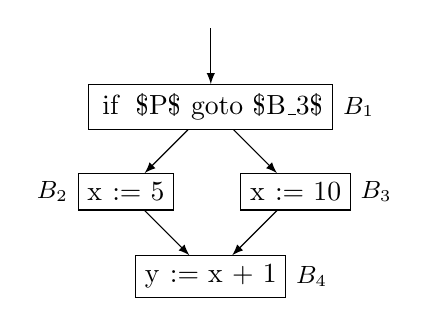
\begin{tikzpicture}[node distance=0.6in,>=latex]
      \node[draw,label=right:{\small $B_1$}] (1) at (0,-1)
        {\lstinline|if $P$ goto $B_3$|};
      \node[draw,label=left:{\small $B_2$}] (2) [below left of=1]
        {\lstinline|x := 5|};
      \node[draw,label=right:{\small $B_3$}] (3) [below right of=1]
        {\lstinline|x := 10|};
      \node[draw,label=right:{\small $B_4$}] (4) [below right of=2]
        {\lstinline|y := x + 1|};

      \draw[->] (0,0) -- (1);
      \draw (1) edge[->] (2)
                edge[->] (3)
            (2) edge[->] (4)
            (3) edge[->] (4);
      \end{tikzpicture}
    \end{minipage}
    \vrule
    \begin{minipage}{0.4\linewidth}
      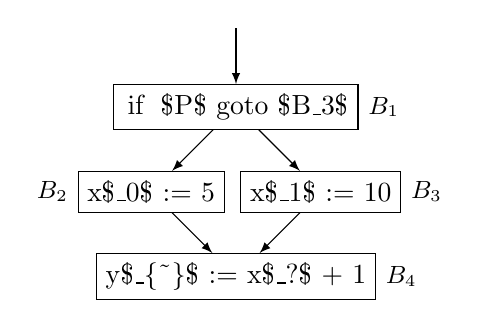
\begin{tikzpicture}[node distance=0.6in,>=latex]
      \node[draw,label=right:{\small $B_1$}] (1) at (0,-1)
        {\lstinline|if $P$ goto $B_3$|};
      \node[draw,label=left:{\small $B_2$}] (2) [below left of=1]
        {\lstinline|x$_0$ := 5|};
      \node[draw,label=right:{\small $B_3$}] (3) [below right of=1]
        {\lstinline|x$_1$ := 10|};
      \node[draw,label=right:{\small $B_4$}] (4) [below right of=2]
        {\lstinline|y$_{~}$ := x$_?$ + 1|};

      \draw[->] (0,0) -- (1);
      \draw (1) edge[->] (2)
                edge[->] (3)
            (2) edge[->] (4)
            (3) edge[->] (4);
      \end{tikzpicture}
    \end{minipage}
  \end{center}
  \end{onlyenv}
  \begin{onlyenv}<2>
  \begin{center}
  \begin{tikzpicture}[node distance=0.7in,>=latex]
  \node[draw,label=right:$B_1$] (1) at (0,-1) {\lstinline|if $P$ goto $B_3$|};
  \node[draw,label=left:$B_2$] (2) [below left of=1] {\lstinline|x$_0$ := 5|};
  \node[draw,label=right:$B_3$] (3) [below right of=1] {\lstinline|x$_1$ := 10|};
  \node[draw,label=right:$B_4$] (4) [below right of=2] {
  \begin{lstlisting}
x$_2$ := $\phi$(x$_0$,x$_1$)
y$_{~}$ := x$_2$ + 1
  \end{lstlisting}
  };

  \draw[->] (0,0) -- (1);
  \draw (1) edge[->] (2)
            edge[->] (3)
        (2) edge[->] (4)
        (3) edge[->] (4);
  \end{tikzpicture}
  \end{center}
  \end{onlyenv}
\end{frame}

\begin{frame}[fragile]{Low-level Representation}{Instructions}
  \begin{itemize}
    \item Code is translated into \verb|insn| objects
    \item Modeled closely after typical assembly-like instructions
    \item Instructions are called on \alert{virtual registers}
  \end{itemize}
  \begin{example}
    \alt<2>{In diagrams}{In Factor syntax}:
    \begin{onlyenv}<1>
      \begin{Verbatim}[gobble=8]
        {
          T{ ##load-integer { dst 867 } { val 1 } }
          T{ ##load-integer { dst 5309 } { val 2 } }
          T{ ##add { dst 31337 } { src1 867 } { src2 5309 } }
        }
      \end{Verbatim}
    \end{onlyenv}
    \begin{onlyenv}<2>
    \begin{center}
    \begin{minipage}{0.5\textwidth}
      \begin{Verbatim}[frame=single,gobble=8]
        ##load-integer 867 1
        ##load-integer 5309 2
        ##add 31337 867 5309
      \end{Verbatim}
    \end{minipage}
    \end{center}
    \end{onlyenv}
  \end{example}
\end{frame}

%\subsection{Optimizations}

%\begin{frame}[fragile]{Optimizations---High-level IR}
%\footnotesize
%\begin{center}
%\begin{minipage}{0.5\linewidth}
%\begin{Verbatim}[commandchars=\\\{\}]
%\PY{k}{:} \PY{n+nf}{optimize-tree} \PY{n+nf}{(} \PY{n+nv}{nodes} \PY{n+nf}{--} \PY{n+nv}{nodes'} \PY{n+nf}{)}
%  [
%      analyze-recursive
%      normalize
%      propagate
%      cleanup
%      \PY{k}{dup }run-escape-analysis? [
%          escape-analysis
%          unbox-tuples
%      ] \PY{k}{when}
%      apply-identities
%      compute-def-use
%      remove-dead-code
%      ?check
%      compute-def-use
%      optimize-modular-arithmetic
%      finalize
%  ] \PY{k}{with-scope ;}
%\end{Verbatim}
%\end{minipage}
%\end{center}
%\end{frame}

\begin{frame}[fragile]{Optimizations}
  \begin{center}
    \begin{minipage}{0.5\linewidth}
      \begin{Verbatim}[gobble=8,commandchars=\\\{\}]
        \PY{k}{:} optimize-cfg ( cfg -- cfg' )
            optimize-tail-calls
            delete-useless-conditionals
            split-branches
            join-blocks
            normalize-height
            construct-ssa
            alias-analysis
            \alert{value-numbering}
            copy-propagation
            eliminate-dead-code \PY{k}{;}
      \end{Verbatim}
    \end{minipage}
  \end{center}
\end{frame}

%\section{Value Numbering}

\begin{frame}{Value Numbering}
  Idea: assign each virtual register a \alert{value number}
  \begin{itemize}
    \item Equal value numbers $\implies$ equal at runtime
    \item Turn recomputations into \texttt{\#\#copy} instructions
  \end{itemize}

  Problem: equivalence is generally undecidable
  \begin{itemize}
    \item Seek \alert{conservative} solution over \alert{Herbrand equivalences}
    \item Consider two values \alert{congruent} if
    \begin{itemize}
      \item They're computed by the same operator
      \item Their operands are congruent
    \end{itemize}
  \end{itemize}
\end{frame}

%\subsection{Local Value Numbering}

\begin{frame}[fragile,t]{Value Numbering}{Implementation}
  \begin{itemize}
    \item \alert{Expressions} are constructed from instructions and value numbers
    \begin{onlyenv}<1>
    \begin{example}
      Suppose\ldots
      \begin{itemize}
        \item virtual register \texttt{2} has the value number \texttt{200}
        \item virtual register \texttt{3} has the value number \texttt{300}
      \end{itemize}
      Then
      \begin{Verbatim}
T{ ##add { dst 1 } { src1 2 } { src2 3 } } >expr
      \end{Verbatim}
      returns
      \begin{Verbatim}
{ ##add 200 300 }
      \end{Verbatim}
    \end{example}
    \end{onlyenv}
    \pause
    \item \alert{Expression graph} = 3 global hash tables
    \begin{itemize}
      \item \texttt{vregs>vns}
      \item \texttt{exprs>vns}
      \item \texttt{vns>insns}
    \end{itemize}
    \item If possible, instructions are simplified using data from expression
    graph
  \end{itemize}
\end{frame}

\begin{frame}{\texttt{value-numbering}}
  \begin{itemize}
    \item Factor currently uses \alert{local} value numbering
    \item Thought to be invented by Balke in the 1960s
    \item Largely credited to Cocke \& Schwartz in the 1970s
    \item \textcolor{green!80!black}{Pros:}
    \begin{itemize}
      \item Easy to understand
      \item Easy to implement
      \item Easy to extend
    \end{itemize}
    \item \alert{Cons:}
    \begin{itemize}
      \item Locality and \alert{pessimism} discover fewer congruences
    \end{itemize}
  \end{itemize}
\end{frame}

\begin{frame}[fragile]{Local Value Numbering}
  \begin{onlyenv}<1>
    \begin{example}[In Factor]
      \factor|0 100 [ 1 fixnum+fast ] times|
    \end{example}
    \begin{example}[In Java]
      \begin{minted}{java}
int i = 0;
for (int j = 0; j < 100; j++) {
  i += 1;
}
      \end{minted}
    \end{example}
  \end{onlyenv}
  \begin{onlyenv}<2>
    \begin{center}
      \includesvg[scale=0.35]{/home/alex/thesis/examples/lvn/7-alias-analysis}
    \end{center}
  \end{onlyenv}
\end{frame}

\begin{frame}[fragile]{Local Value Numbering}{Basic Block 1}
  \begin{onlyenv}<1>
  \begin{Verbatim}
vregs>vns = H{ }
exprs>vns = H{ }
  \end{Verbatim}
  \end{onlyenv}
  \begin{onlyenv}<2>
  \begin{Verbatim}
vregs>vns = H{ { 21 21 } }
exprs>vns = H{ {  0 21 } }
  \end{Verbatim}
  \end{onlyenv}
  \begin{onlyenv}<3>
  \begin{Verbatim}
vregs>vns = H{ { 21 21 } {  22 22 } }
exprs>vns = H{ {  0 21 } { 100 22 } }
  \end{Verbatim}
  \end{onlyenv}
  \begin{onlyenv}<4>
  \begin{Verbatim}
vregs>vns = H{ { 21 21 } {  22 22 } { 23 21 } }
exprs>vns = H{ {  0 21 } { 100 22 } }
  \end{Verbatim}
  \end{onlyenv}
  \begin{onlyenv}<5>
  \begin{Verbatim}
vregs>vns = H{ { 21 21 } {  22 22 } { 23 21 } { 24 22 } ... }
exprs>vns = H{ {  0 21 } { 100 22 } }
  \end{Verbatim}
  \end{onlyenv}
  \begin{columns}[t,onlytextwidth]
    \begin{column}[t]{.45\textwidth}
      \begin{onlyenv}<1-4>
      \begin{Verbatim}[frame=single]
##inc-d 3
##load-integer 21 0
##load-integer 22 100
##load-integer 23 0
##copy 24 22 any-rep
##copy 25 21 any-rep
##copy 26 24 any-rep
##copy 27 23 any-rep
##branch
      \end{Verbatim}
      \end{onlyenv}
      \begin{onlyenv}<5->
      \begin{Verbatim}[frame=single]
##inc-d 3
##load-integer 21 0
##load-integer 22 100
##copy 23 21 any-rep
##copy 24 22 any-rep
##copy 25 21 any-rep
##copy 26 24 any-rep
##copy 27 23 any-rep
##branch
      \end{Verbatim}
      \end{onlyenv}
    \end{column}

    \begin{column}[t]{.5\textwidth}
      \begin{onlyenv}<1>
        \begin{Verbatim}
(no-op)
        \end{Verbatim}
      \end{onlyenv}
      \begin{onlyenv}<2>
        \begin{Verbatim}
(no-op)
>expr = 0
        \end{Verbatim}
      \end{onlyenv}
      \begin{onlyenv}<3>
        \begin{Verbatim}
(no-op)
>expr = 0
>expr = 100
        \end{Verbatim}
      \end{onlyenv}
      \begin{onlyenv}<4>
        \begin{Verbatim}
(no-op)
>expr = 0
>expr = 100
>expr = 0
        \end{Verbatim}
      \end{onlyenv}
      \begin{onlyenv}<5>
        \begin{Verbatim}
(no-op)
>expr = 0
>expr = 100
>expr = 0
...
...
...
...
        \end{Verbatim}
      \end{onlyenv}
    \end{column}
  \end{columns}
\end{frame}

\begin{frame}[fragile]{Local Value Numbering}{Basic Block 2}
  \begin{onlyenv}<1>
  \begin{Verbatim}
vregs>vns = H{ }
exprs>vns = H{ }
  \end{Verbatim}
  \end{onlyenv}
  \begin{onlyenv}<2>
  \begin{Verbatim}
vregs>vns = H{ { 30 30 } { 26 26 } { 31 31 } }
exprs>vns = H{ { { ##compare-integer 30 26 cc< } 31 } }
  \end{Verbatim}
  \end{onlyenv}
  \begin{onlyenv}<3->
  \begin{Verbatim}
vregs>vns = H{ { 30 30 } { 26 26 } { 31 31 } { 32 31 } ... }
exprs>vns = H{ { { ##compare-integer 30 26 cc< } 31 } }
  \end{Verbatim}
  \end{onlyenv}
  \begin{columns}[t,onlytextwidth]
    \begin{column}[t]{.6\textwidth}
      \begin{onlyenv}<1-3>
      \begin{Verbatim}[frame=single]
##phi 29 H{ { 1 25 } { 3 41 } }
##phi 30 H{ { 1 27 } { 3 42 } }
##compare-integer 31 30 26 cc< 9
##copy 32 31 any-rep
##copy 33 26 any-rep
##copy 34 31 any-rep
##compare-imm-branch 32 f cc/=
      \end{Verbatim}
      \end{onlyenv}
      \begin{onlyenv}<4->
      \begin{Verbatim}[frame=single]
##phi 29 H{ { 1 25 } { 3 41 } }
##phi 30 H{ { 1 27 } { 3 42 } }
##compare-integer 31 30 26 cc< 9
##copy 32 31 any-rep
##copy 33 26 any-rep
##copy 34 31 any-rep
##compare-integer-branch 30 26 cc<
      \end{Verbatim}
      \end{onlyenv}
    \end{column}

    \begin{column}[t]{.3\textwidth}
      \begin{onlyenv}<1>
        \begin{Verbatim}
(no-op)
(no-op)
        \end{Verbatim}
      \end{onlyenv}
      \begin{onlyenv}<2>
        \begin{Verbatim}
(no-op)
(no-op)
>expr = ...
        \end{Verbatim}
      \end{onlyenv}
      \begin{onlyenv}<3->
        \begin{Verbatim}
(no-op)
(no-op)
>expr = ...
...
...
...
        \end{Verbatim}
      \end{onlyenv}
    \end{column}
  \end{columns}
\end{frame}

\begin{frame}[fragile]{Local Value Numbering}{Basic Block 3}
  \begin{onlyenv}<1>
  \begin{Verbatim}
vregs>vns = H{ }
exprs>vns = H{ }
  \end{Verbatim}
  \end{onlyenv}
  \begin{onlyenv}<2>
  \begin{Verbatim}
vregs>vns = H{ { 35 35 } }
exprs>vns = H{ {  1 35 } }
  \end{Verbatim}
  \end{onlyenv}
  \begin{onlyenv}<3>
  \begin{Verbatim}
vregs>vns = H{ { 35 35 } { 29 29 } { 36 36 } }
exprs>vns = H{ {  1 35 } { { ##add-imm 29 1 } 36 } }
  \end{Verbatim}
  \end{onlyenv}
  \begin{onlyenv}<4>
  \begin{Verbatim}
vregs>vns = H{ { 35 35 } { 29 29 } { 36 36 }  { 37 35 } }
exprs>vns = H{ {  1 35 } { { ##add-imm 29 1 } 36 } }
  \end{Verbatim}
  \end{onlyenv}
  \begin{onlyenv}<5->
  \begin{Verbatim}
vregs>vns = H{ { 35 35 } { 29 29 } { 36 36 }  { 37 35 } ... }
exprs>vns = H{ {  1 35 } { { ##add-imm 29 1 } 36 } ... }
  \end{Verbatim}
  \end{onlyenv}
  \begin{columns}[t,onlytextwidth]
    \begin{column}[t]{.4\textwidth}
      \begin{onlyenv}<1-3>
      \begin{Verbatim}[frame=single]
##load-integer 35 1
##add 36 29 35
##load-integer 37 1
##add 38 30 37
##copy 39 30 any-rep
##copy 40 26 any-rep
##copy 41 36 any-rep
##copy 42 38 any-rep
##branch
      \end{Verbatim}
      \end{onlyenv}
      \begin{onlyenv}<4>
      \begin{Verbatim}[frame=single]
##load-integer 35 1
##add-imm 36 29 1
##load-integer 37 1
##add 38 30 37
##copy 39 30 any-rep
##copy 40 26 any-rep
##copy 41 36 any-rep
##copy 42 38 any-rep
##branch
      \end{Verbatim}
      \end{onlyenv}
      \begin{onlyenv}<5>
      \begin{Verbatim}[frame=single]
##load-integer 35 1
##add-imm 36 29 1
##copy 37 35 any-rep
##add 38 30 37
##copy 39 30 any-rep
##copy 40 26 any-rep
##copy 41 36 any-rep
##copy 42 38 any-rep
##branch
      \end{Verbatim}
      \end{onlyenv}
      \begin{onlyenv}<6->
      \begin{Verbatim}[frame=single]
##load-integer 35 1
##add-imm 36 29 1
##copy 37 35 any-rep
##add-imm 38 30 1
##copy 39 30 any-rep
##copy 40 26 any-rep
##copy 41 36 any-rep
##copy 42 38 any-rep
##branch
      \end{Verbatim}
      \end{onlyenv}
    \end{column}

    \begin{column}[t]{.5\textwidth}
      \begin{onlyenv}<2>
        \begin{Verbatim}
>expr = 1
        \end{Verbatim}
      \end{onlyenv}
      \begin{onlyenv}<3>
        \begin{Verbatim}
>expr = 1
>expr = { ##add-imm 29 1 }
        \end{Verbatim}
      \end{onlyenv}
      \begin{onlyenv}<4>
        \begin{Verbatim}
>expr = 1
>expr = { ##add-imm 29 1 }
>expr = 1
        \end{Verbatim}
      \end{onlyenv}
      \begin{onlyenv}<5>
        \begin{Verbatim}
>expr = 1
>expr = { ##add-imm 29 1 }
>expr = 1
>expr = { ##add-imm 30 1 }
        \end{Verbatim}
      \end{onlyenv}
      \begin{onlyenv}<6->
        \begin{Verbatim}
>expr = 1
>expr = { ##add-imm 29 1 }
>expr = 1
>expr = { ##add-imm 30 1 }
...
...
...
...
        \end{Verbatim}
      \end{onlyenv}
    \end{column}
  \end{columns}
\end{frame}

\begin{frame}{Local Value Numbering Results}
  \begin{center}
    \includesvg[scale=0.5]{/home/alex/thesis/examples/lvn/11-finalize-cfg}
  \end{center}
\end{frame}

%\subsection{Global Value Numbering}

\begin{frame}[fragile]{Same Example, Global Algorithm}
  Changes:
  \begin{itemize}
    \item \alert{Global}---don't wipe out hash tables after each block
    \item \alert{Optimistic}---previously unseen values considered redundant
    \item \alert{Fixed point} iteration---optimism may be wrong first time
          around
    \item \alert{Offline} replacements---only on final pass
  \end{itemize}
  \begin{definition}[Notation]
    \begin{align*}
      \vn{n} &= \{\vreg{x}, \vreg{y}, \vreg{z}\} \tag{\texttt{expr}}
    \end{align*}
    versus
    \begin{center}
    \begin{minipage}{0.5\linewidth}
    \begin{Verbatim}
vregs>vns = H{ { x n } { y n } { z n } }
exprs>vns = H{ { expr n } }
    \end{Verbatim}
    \end{minipage}
    \end{center}
  \end{definition}
\end{frame}

\begin{frame}[fragile]{Global Value Numbering}{Iteration 1, Basic Block 1}
  \footnotesize
  \begin{columns}[t,onlytextwidth]
    \begin{column}[t]{.5\textwidth}
      \begin{onlyenv}<1>
        \begin{Verbatim}[frame=single,commandchars=\\\{\}]
##inc-d 3
##load-integer 21 0
##load-integer 22 100
##load-integer 23 0
##copy 24 22 any-rep
##copy 25 21 any-rep
##copy 26 24 any-rep
##copy 27 23 any-rep
##branch
        \end{Verbatim}
      \end{onlyenv}
      \begin{onlyenv}<2>
        \begin{Verbatim}[frame=single,commandchars=\\\{\}]
##inc-d 3
\alert{##load-integer 21 0}
##load-integer 22 100
##load-integer 23 0
##copy 24 22 any-rep
##copy 25 21 any-rep
##copy 26 24 any-rep
##copy 27 23 any-rep
##branch
        \end{Verbatim}
      \end{onlyenv}
      \begin{onlyenv}<3>
        \begin{Verbatim}[frame=single,commandchars=\\\{\}]
##inc-d 3
##load-integer 21 0
\alert{##load-integer 22 100}
##load-integer 23 0
##copy 24 22 any-rep
##copy 25 21 any-rep
##copy 26 24 any-rep
##copy 27 23 any-rep
##branch
        \end{Verbatim}
      \end{onlyenv}
      \begin{onlyenv}<4>
        \begin{Verbatim}[frame=single,commandchars=\\\{\}]
##inc-d 3
##load-integer 21 0
##load-integer 22 100
\alert{##load-integer 23 0}
##copy 24 22 any-rep
##copy 25 21 any-rep
##copy 26 24 any-rep
##copy 27 23 any-rep
##branch
        \end{Verbatim}
      \end{onlyenv}
      \begin{onlyenv}<5>
        \begin{Verbatim}[frame=single,commandchars=\\\{\}]
##inc-d 3
##load-integer 21 0
##load-integer 22 100
##load-integer 23 0
\alert{##copy 24 22 any-rep}
\alert{##copy 25 21 any-rep}
\alert{##copy 26 24 any-rep}
\alert{##copy 27 23 any-rep}
##branch
        \end{Verbatim}
      \end{onlyenv}
    \end{column}
    \begin{column}{.5\textwidth}
      \begin{onlyenv}<1>
        \begin{align*}
          \vn{\textbf{f}} &= U \tag{everything} \\
        \end{align*}
      \end{onlyenv}
      \begin{onlyenv}<2>
        \begin{align*}
          \alert{\vn{21}} &= \alert{\{\vreg{21}\}} \tag{\alert{\texttt{0}}} \\
        \end{align*}
      \end{onlyenv}
      \begin{onlyenv}<3>
        \begin{align*}
          \vn{21} &= \{\vreg{21}\} \tag{\texttt{0}}   \\
          \alert{\vn{22}} &= \alert{\{\vreg{22}\}} \tag{\alert{\texttt{100}}} \\
        \end{align*}
      \end{onlyenv}
      \begin{onlyenv}<4>
        \begin{align*}
          \vn{21} &= \{\vreg{21},\alert{\vreg{23}}\} \tag{\texttt{0}}   \\
          \vn{22} &= \{\vreg{22}\}           \tag{\texttt{100}} \\
        \end{align*}
      \end{onlyenv}
      \begin{onlyenv}<5>
        \begin{align*}
          \vn{21} &= \{\vreg{21}, \vreg{23}, \alert{\vreg{25}}, \alert{\vreg{27}}\} \tag{\texttt{0}}   \\
          \vn{22} &= \{\vreg{22}, \alert{\vreg{24}}, \alert{\vreg{26}}\}            \tag{\texttt{100}} \\
        \end{align*}
      \end{onlyenv}
    \end{column}
  \end{columns}
\end{frame}

\begin{frame}[fragile]{Global Value Numbering}{Iteration 1, Basic Block 2}
  \footnotesize
  \begin{columns}[t,onlytextwidth]
    \begin{column}[t]{.5\textwidth}
      \begin{onlyenv}<1>
        \begin{Verbatim}[frame=single,commandchars=\\\{\}]
##phi 29 H\{ \{ 1 25 \} \{ 3 41 \} \}
##phi 30 H\{ \{ 1 27 \} \{ 3 42 \} \}
##compare-integer 31 30 26 cc< 9
##copy 32 31 any-rep
##copy 33 26 any-rep
##copy 34 31 any-rep
##compare-imm-branch 32 f cc/=
        \end{Verbatim}
      \end{onlyenv}
      \begin{onlyenv}<2>
        \begin{Verbatim}[frame=single,commandchars=\\\{\}]
\alert{##phi 29 H\{ \{ 1 25 \} \{ 3 41 \} \}}
##phi 30 H\{ \{ 1 27 \} \{ 3 42 \} \}
##compare-integer 31 30 26 cc< 9
##copy 32 31 any-rep
##copy 33 26 any-rep
##copy 34 31 any-rep
##compare-imm-branch 32 f cc/=
        \end{Verbatim}
      \end{onlyenv}
      \begin{onlyenv}<3>
        \begin{Verbatim}[frame=single,commandchars=\\\{\}]
##phi 29 H\{ \{ 1 25 \} \{ 3 41 \} \}
\alert{##phi 30 H\{ \{ 1 27 \} \{ 3 42 \} \}}
##compare-integer 31 30 26 cc< 9
##copy 32 31 any-rep
##copy 33 26 any-rep
##copy 34 31 any-rep
##compare-imm-branch 32 f cc/=
        \end{Verbatim}
      \end{onlyenv}
      \begin{onlyenv}<4>
        \begin{Verbatim}[frame=single,commandchars=\\\{\}]
##phi 29 H\{ \{ 1 25 \} \{ 3 41 \} \}
##phi 30 H\{ \{ 1 27 \} \{ 3 42 \} \}
\alert{##compare-integer 31 30 26 cc< 9}
##copy 32 31 any-rep
##copy 33 26 any-rep
##copy 34 31 any-rep
##compare-imm-branch 32 f cc/=
        \end{Verbatim}
      \end{onlyenv}
      \begin{onlyenv}<5->
        \begin{Verbatim}[frame=single,commandchars=\\\{\}]
##phi 29 H\{ \{ 1 25 \} \{ 3 41 \} \}
##phi 30 H\{ \{ 1 27 \} \{ 3 42 \} \}
##compare-integer 31 30 26 cc< 9
\alert{##copy 32 31 any-rep}
\alert{##copy 33 26 any-rep}
\alert{##copy 34 31 any-rep}
##compare-imm-branch 32 f cc/=
        \end{Verbatim}
      \end{onlyenv}
    \end{column}
    \begin{column}{.5\textwidth}
      \begin{onlyenv}<1>
        \begin{align*}
          \vn{21} &= \{\vreg{21}, \vreg{23}, \vreg{25}, \vreg{27}\} \tag{\texttt{0}}   \\
          \vn{22} &= \{\vreg{22}, \vreg{24}, \vreg{26}\}            \tag{\texttt{100}} \\
        \end{align*}
      \end{onlyenv}
      \begin{onlyenv}<2>
        \begin{align*}
          \vn{21} &= \{\vreg{21}, \vreg{23}, \vreg{25}, \vreg{27}, \alert{\vreg{29}}\} \tag{\texttt{0}}   \\
          \vn{22} &= \{\vreg{22}, \vreg{24}, \vreg{26}\}            \tag{\texttt{100}} \\
        \end{align*}
      \end{onlyenv}
      \begin{onlyenv}<3>
        \begin{align*}
          \vn{21} &= \{\vreg{21}, \vreg{23}, \vreg{25}, \vreg{27}, \vreg{29}, \alert{\vreg{30}}\} \tag{\texttt{0}}   \\
          \vn{22} &= \{\vreg{22}, \vreg{24}, \vreg{26}\}            \tag{\texttt{100}} \\
        \end{align*}
      \end{onlyenv}
      \begin{onlyenv}<4>
        \begin{align*}
          \vn{21} &= \{\vreg{21}, \vreg{23}, \vreg{25}, \vreg{27}, \vreg{29}, \vreg{30}\} \tag{\texttt{0}}   \\
          \vn{22} &= \{\vreg{22}, \vreg{24}, \vreg{26}\}            \tag{\texttt{100}} \\
          \alert{\vn{31}} &= \alert{\{\vreg{31}\}}                                  \tag{\alert{\texttt{\textbf{t}}}} \\
        \end{align*}
      \end{onlyenv}
      \begin{onlyenv}<5>
        \begin{align*}
          \vn{21} &= \{\vreg{21},
                       \vreg{23},
                       \vreg{25},
                       \vreg{27},
                       \vreg{29},
                       \vreg{30}\} \tag{\texttt{0}} \\
          \vn{22} &= \{\vreg{22},
                       \vreg{24},
                       \vreg{26},
                       \alert{\vreg{33}}\} \tag{\texttt{100}} \\
          \vn{31} &= \{\vreg{31},
                       \alert{\vreg{32}},
                       \alert{\vreg{34}}\} \tag{\texttt{\textbf{t}}}
        \end{align*}
      \end{onlyenv}
    \end{column}
  \end{columns}
\end{frame}

\begin{frame}[fragile]{Global Value Numbering}{Iteration 1, Basic Block 3}
  \footnotesize
  \begin{columns}[t,onlytextwidth]
    \begin{column}[t]{.5\textwidth}
      \begin{onlyenv}<1>
        \begin{Verbatim}[frame=single,commandchars=\\\{\}]
##load-integer 35 1
##add 36 29 35
##load-integer 37 1
##add 38 30 37
##copy 39 30 any-rep
##copy 40 26 any-rep
##copy 41 36 any-rep
##copy 42 38 any-rep
##branch
        \end{Verbatim}
      \end{onlyenv}
      \begin{onlyenv}<2>
        \begin{Verbatim}[frame=single,commandchars=\\\{\}]
\alert{##load-integer 35 1}
##add 36 29 35
##load-integer 37 1
##add 38 30 37
##copy 39 30 any-rep
##copy 40 26 any-rep
##copy 41 36 any-rep
##copy 42 38 any-rep
##branch
        \end{Verbatim}
      \end{onlyenv}
      \begin{onlyenv}<3>
        \begin{Verbatim}[frame=single,commandchars=\\\{\}]
##load-integer 35 1
\alert{##add 36 29 35}
##load-integer 37 1
##add 38 30 37
##copy 39 30 any-rep
##copy 40 26 any-rep
##copy 41 36 any-rep
##copy 42 38 any-rep
##branch
        \end{Verbatim}
      \end{onlyenv}
      \begin{onlyenv}<4>
        \begin{Verbatim}[frame=single,commandchars=\\\{\}]
##load-integer 35 1
##add 36 29 35
\alert{##load-integer 37 1}
##add 38 30 37
##copy 39 30 any-rep
##copy 40 26 any-rep
##copy 41 36 any-rep
##copy 42 38 any-rep
##branch
        \end{Verbatim}
      \end{onlyenv}
      \begin{onlyenv}<5>
        \begin{Verbatim}[frame=single,commandchars=\\\{\}]
##load-integer 35 1
##add 36 29 35
##load-integer 37 1
\alert{##add 38 30 37}
##copy 39 30 any-rep
##copy 40 26 any-rep
##copy 41 36 any-rep
##copy 42 38 any-rep
##branch
        \end{Verbatim}
      \end{onlyenv}
      \begin{onlyenv}<6>
        \begin{Verbatim}[frame=single,commandchars=\\\{\}]
##load-integer 35 1
##add 36 29 35
##load-integer 37 1
##add 38 30 37
\alert{##copy 39 30 any-rep}
\alert{##copy 40 26 any-rep}
\alert{##copy 41 36 any-rep}
\alert{##copy 42 38 any-rep}
##branch
        \end{Verbatim}
      \end{onlyenv}
    \end{column}
    \begin{column}{.5\textwidth}
      \begin{onlyenv}<1>
        \begin{align*}
          \vn{21} &= \{\vreg{21},
                       \vreg{23},
                       \vreg{25},
                       \vreg{27},
                       \vreg{29},
                       \vreg{30}\} \tag{\texttt{0}} \\
          \vn{22} &= \{\vreg{22},
                       \vreg{24},
                       \vreg{26},
                       \vreg{33}\} \tag{\texttt{100}} \\
          \vn{31} &= \{\vreg{31},
                       \vreg{32},
                       \vreg{34}\} \tag{\texttt{\textbf{t}}}
        \end{align*}
      \end{onlyenv}
      \begin{onlyenv}<2>
        \begin{align*}
          \vn{21} &= \{\vreg{21},
                       \vreg{23},
                       \vreg{25},
                       \vreg{27},
                       \vreg{29},
                       \vreg{30}\} \tag{\texttt{0}} \\
          \vn{22} &= \{\vreg{22},
                       \vreg{24},
                       \vreg{26},
                       \vreg{33}\} \tag{\texttt{100}} \\
          \vn{31} &= \{\vreg{31},
                       \vreg{32},
                       \vreg{34}\} \tag{\texttt{\textbf{t}}} \\
          \alert{\vn{35}} &= \alert{\{\vreg{35}\}} \tag{\alert{\texttt{1}}}
        \end{align*}
      \end{onlyenv}
      \begin{onlyenv}<3>
        \begin{align*}
          \vn{21} &= \{\vreg{21},
                       \vreg{23},
                       \vreg{25},
                       \vreg{27},
                       \vreg{29},
                       \vreg{30}\} \tag{\texttt{0}} \\
          \vn{22} &= \{\vreg{22},
                       \vreg{24},
                       \vreg{26},
                       \vreg{33}\} \tag{\texttt{100}} \\
          \vn{31} &= \{\vreg{31},
                       \vreg{32},
                       \vreg{34}\} \tag{\texttt{\textbf{t}}} \\
          \vn{35} &= \{\vreg{35},
                       \alert{\vreg{36}}\} \tag{\texttt{1}}
        \end{align*}
      \end{onlyenv}
      \begin{onlyenv}<4>
        \begin{align*}
          \vn{21} &= \{\vreg{21},
                       \vreg{23},
                       \vreg{25},
                       \vreg{27},
                       \vreg{29},
                       \vreg{30}\} \tag{\texttt{0}} \\
          \vn{22} &= \{\vreg{22},
                       \vreg{24},
                       \vreg{26},
                       \vreg{33}\} \tag{\texttt{100}} \\
          \vn{31} &= \{\vreg{31},
                       \vreg{32},
                       \vreg{34}\} \tag{\texttt{\textbf{t}}} \\
          \vn{35} &= \{\vreg{35},
                       \vreg{36},
                       \alert{\vreg{37}}\} \tag{\texttt{1}}
        \end{align*}
      \end{onlyenv}
      \begin{onlyenv}<5>
        \begin{align*}
          \vn{21} &= \{\vreg{21},
                       \vreg{23},
                       \vreg{25},
                       \vreg{27},
                       \vreg{29},
                       \vreg{30}\} \tag{\texttt{0}} \\
          \vn{22} &= \{\vreg{22},
                       \vreg{24},
                       \vreg{26},
                       \vreg{33}\} \tag{\texttt{100}} \\
          \vn{31} &= \{\vreg{31},
                       \vreg{32},
                       \vreg{34}\} \tag{\texttt{\textbf{t}}} \\
          \vn{35} &= \{\vreg{35},
                       \vreg{36},
                       \vreg{37},
                       \alert{\vreg{38}}\} \tag{\texttt{1}}
        \end{align*}
      \end{onlyenv}
      \begin{onlyenv}<6>
        \begin{align*}
          \vn{21} &= \{\vreg{21},
                       \vreg{23},
                       \vreg{25},
                       \vreg{27},
                       \vreg{29},
                       \vreg{30},
                       \alert{\vreg{39}}\} \tag{\texttt{0}} \\
          \vn{22} &= \{\vreg{22},
                       \vreg{24},
                       \vreg{26},
                       \vreg{33},
                       \alert{\vreg{40}}\} \tag{\texttt{100}} \\
          \vn{31} &= \{\vreg{31},
                       \vreg{32},
                       \vreg{34}\} \tag{\texttt{\textbf{t}}} \\
          \vn{35} &= \{\vreg{35},
                       \vreg{36},
                       \vreg{37},
                       \vreg{38},
                       \alert{\vreg{41}},
                       \alert{\vreg{42}}\} \tag{\texttt{1}}
        \end{align*}
      \end{onlyenv}
    \end{column}
  \end{columns}
\end{frame}

\begin{frame}[fragile]{Global Value Numbering}{Iteration 2, Basic Block 1}
  \footnotesize
  \begin{columns}[t,onlytextwidth]
    \begin{column}[t]{.5\textwidth}
      % okay to not highlight anything
      \begin{Verbatim}[frame=single]
##inc-d 3
##load-integer 21 0
##load-integer 22 100
##load-integer 23 0
##copy 24 22 any-rep
##copy 25 21 any-rep
##copy 26 24 any-rep
##copy 27 23 any-rep
##branch
      \end{Verbatim}
    \end{column}
    \begin{column}{.5\textwidth}
      \begin{onlyenv}<1>
        \begin{align*}
          \vn{21} &= \{\vreg{21},
                       \vreg{23},
                       \vreg{25},
                       \vreg{27},
                       \vreg{29},
                       \vreg{30},
                       \vreg{39}\} \tag{\alert{---}} \\
          \vn{22} &= \{\vreg{22},
                       \vreg{24},
                       \vreg{26},
                       \vreg{33},
                       \vreg{40}\} \tag{\alert{---}} \\
          \vn{31} &= \{\vreg{31},
                       \vreg{32},
                       \vreg{34}\} \tag{\alert{---}} \\
          \vn{35} &= \{\vreg{35},
                       \vreg{36},
                       \vreg{37},
                       \vreg{38},
                       \vreg{41},
                       \vreg{42}\} \tag{\alert{---}}
        \end{align*}
      \end{onlyenv}
      \begin{onlyenv}<2>
        \begin{align*}
          \vn{21} &= \{\vreg{21},
                       \vreg{23},
                       \vreg{25},
                       \vreg{27},
                       \vreg{29},
                       \vreg{30},
                       \vreg{39}\} \tag{\alert{\texttt{0}}} \\
          \vn{22} &= \{\vreg{22},
                       \vreg{24},
                       \vreg{26},
                       \vreg{33},
                       \vreg{40}\} \tag{\alert{\texttt{100}}} \\
          \vn{31} &= \{\vreg{31},
                       \vreg{32},
                       \vreg{34}\} \tag{---} \\
          \vn{35} &= \{\vreg{35},
                       \vreg{36},
                       \vreg{37},
                       \vreg{38},
                       \vreg{41},
                       \vreg{42}\} \tag{---}
        \end{align*}
      \end{onlyenv}
    \end{column}
  \end{columns}
\end{frame}

\begin{frame}[fragile]{Global Value Numbering}{Iteration 2, Basic Block 2}
  \footnotesize
  \begin{columns}[t,onlytextwidth]
    \begin{column}[t]{.5\textwidth}
      \begin{onlyenv}<1>
        \begin{Verbatim}[frame=single,commandchars=\\\{\}]
##phi 29 H\{ \{ 1 25 \} \{ 3 41 \} \}
##phi 30 H\{ \{ 1 27 \} \{ 3 42 \} \}
##compare-integer 31 30 26 cc< 9
##copy 32 31 any-rep
##copy 33 26 any-rep
##copy 34 31 any-rep
##compare-imm-branch 32 f cc/=
        \end{Verbatim}
      \end{onlyenv}
      \begin{onlyenv}<2>
        \begin{Verbatim}[frame=single,commandchars=\\\{\}]
\alert{##phi 29 H\{ \{ 1 25 \} \{ 3 41 \} \}}
##phi 30 H\{ \{ 1 27 \} \{ 3 42 \} \}
##compare-integer 31 30 26 cc< 9
##copy 32 31 any-rep
##copy 33 26 any-rep
##copy 34 31 any-rep
##compare-imm-branch 32 f cc/=
        \end{Verbatim}
      \end{onlyenv}
      \begin{onlyenv}<3>
        \begin{Verbatim}[frame=single,commandchars=\\\{\}]
##phi 29 H\{ \{ 1 25 \} \{ 3 41 \} \}
\alert{##phi 30 H\{ \{ 1 27 \} \{ 3 42 \} \}}
##compare-integer 31 30 26 cc< 9
##copy 32 31 any-rep
##copy 33 26 any-rep
##copy 34 31 any-rep
##compare-imm-branch 32 f cc/=
        \end{Verbatim}
      \end{onlyenv}
      \begin{onlyenv}<4>
        \begin{Verbatim}[frame=single,commandchars=\\\{\}]
##phi 29 H\{ \{ 1 25 \} \{ 3 41 \} \}
##phi 30 H\{ \{ 1 27 \} \{ 3 42 \} \}
\alert{##compare-integer 31 30 26 cc< 9}
\alert{##copy 32 31 any-rep}
\alert{##copy 33 26 any-rep}
\alert{##copy 34 31 any-rep}
##compare-imm-branch 32 f cc/=
        \end{Verbatim}
      \end{onlyenv}
    \end{column}
    \begin{column}{.5\textwidth}
      \begin{onlyenv}<1>
        \begin{align*}
          \vn{21} &= \{\vreg{21},
                       \vreg{23},
                       \vreg{25},
                       \vreg{27},
                       \vreg{29},
                       \vreg{30},
                       \vreg{39}\} \tag{\texttt{0}} \\
          \vn{22} &= \{\vreg{22},
                       \vreg{24},
                       \vreg{26},
                       \vreg{33},
                       \vreg{40}\} \tag{\texttt{100}} \\
          \vn{31} &= \{\vreg{31},
                       \vreg{32},
                       \vreg{34}\} \tag{---} \\
          \vn{35} &= \{\vreg{35},
                       \vreg{36},
                       \vreg{37},
                       \vreg{38},
                       \vreg{41},
                       \vreg{42}\} \tag{---}
        \end{align*}
      \end{onlyenv}
      \begin{onlyenv}<2>
        \begin{align*}
          \vn{21} &= \{\vreg{21},
                       \vreg{23},
                       \vreg{25},
                       \vreg{27},
                       \vreg{30},
                       \vreg{39}\} \tag{\texttt{0}} \\
          \vn{22} &= \{\vreg{22},
                       \vreg{24},
                       \vreg{26},
                       \vreg{33},
                       \vreg{40}\} \tag{\texttt{100}} \\
          \alert{\vn{29}} &= \alert{\{\vreg{29}\}} \tag{\alert{\texttt{\#\#phi 2 21 35}}} \\
          \vn{31} &= \{\vreg{31},
                       \vreg{32},
                       \vreg{34}\} \tag{---} \\
          \vn{35} &= \{\vreg{35},
                       \vreg{36},
                       \vreg{37},
                       \vreg{38},
                       \vreg{41},
                       \vreg{42}\} \tag{---}
        \end{align*}
      \end{onlyenv}
      \begin{onlyenv}<3>
        \begin{align*}
          \vn{21} &= \{\vreg{21},
                       \vreg{23},
                       \vreg{25},
                       \vreg{27},
                       \vreg{39}\} \tag{\texttt{0}} \\
          \vn{22} &= \{\vreg{22},
                       \vreg{24},
                       \vreg{26},
                       \vreg{33},
                       \vreg{40}\} \tag{\texttt{100}} \\
          \vn{29} &= \{\vreg{29},
                       \alert{\vreg{30}}\} \tag{\texttt{\#\#phi 2 21 35}} \\
          \vn{31} &= \{\vreg{31},
                       \vreg{32},
                       \vreg{34}\} \tag{---} \\
          \vn{35} &= \{\vreg{35},
                       \vreg{36},
                       \vreg{37},
                       \vreg{38},
                       \vreg{41},
                       \vreg{42}\} \tag{---}
        \end{align*}
      \end{onlyenv}
      \begin{onlyenv}<4>
        \begin{align*}
          \vn{21} &= \{\vreg{21},
                       \vreg{23},
                       \vreg{25},
                       \vreg{27},
                       \vreg{39}\} \tag{\texttt{0}} \\
          \vn{22} &= \{\vreg{22},
                       \vreg{24},
                       \vreg{26},
                       \vreg{33},
                       \vreg{40}\} \tag{\texttt{100}} \\
          \vn{29} &= \{\vreg{29},
                       \vreg{30}\} \tag{\texttt{\#\#phi 2 21 35}} \\
          \vn{31} &= \{\vreg{31},
                       \vreg{32},
                       \vreg{34}\} \tag{\alert{\texttt{cmp 29 100 cc<}}} \\
          \vn{35} &= \{\vreg{35},
                       \vreg{36},
                       \vreg{37},
                       \vreg{38},
                       \vreg{41},
                       \vreg{42}\} \tag{---}
        \end{align*}
      \end{onlyenv}
    \end{column}
  \end{columns}
\end{frame}

\begin{frame}[fragile]{Global Value Numbering}{Iteration 2, Basic Block 3}
  \footnotesize
  \begin{columns}[t,onlytextwidth]
    \begin{column}[t]{.5\textwidth}
      \begin{onlyenv}<1>
        \begin{Verbatim}[frame=single,commandchars=\\\{\}]
##load-integer 35 1
##add 36 29 35
##load-integer 37 1
##add 38 30 37
##copy 39 30 any-rep
##copy 40 26 any-rep
##copy 41 36 any-rep
##copy 42 38 any-rep
##branch
        \end{Verbatim}
      \end{onlyenv}
      \begin{onlyenv}<2>
        \begin{Verbatim}[frame=single,commandchars=\\\{\}]
\alert{##load-integer 35 1}
##add 36 29 35
##load-integer 37 1
##add 38 30 37
##copy 39 30 any-rep
##copy 40 26 any-rep
##copy 41 36 any-rep
##copy 42 38 any-rep
##branch
        \end{Verbatim}
      \end{onlyenv}
      \begin{onlyenv}<3>
        \begin{Verbatim}[frame=single,commandchars=\\\{\}]
##load-integer 35 1
\alert{##add 36 29 35}
##load-integer 37 1
##add 38 30 37
##copy 39 30 any-rep
##copy 40 26 any-rep
##copy 41 36 any-rep
##copy 42 38 any-rep
##branch
        \end{Verbatim}
      \end{onlyenv}
      \begin{onlyenv}<4>
        \begin{Verbatim}[frame=single,commandchars=\\\{\}]
##load-integer 35 1
##add 36 29 35
\alert{##load-integer 37 1}
##add 38 30 37
##copy 39 30 any-rep
##copy 40 26 any-rep
##copy 41 36 any-rep
##copy 42 38 any-rep
##branch
        \end{Verbatim}
      \end{onlyenv}
      \begin{onlyenv}<5>
        \begin{Verbatim}[frame=single,commandchars=\\\{\}]
##load-integer 35 1
##add 36 29 35
##load-integer 37 1
\alert{##add 38 30 37}
##copy 39 30 any-rep
##copy 40 26 any-rep
##copy 41 36 any-rep
##copy 42 38 any-rep
##branch
        \end{Verbatim}
      \end{onlyenv}
      \begin{onlyenv}<6>
        \begin{Verbatim}[frame=single,commandchars=\\\{\}]
##load-integer 35 1
##add 36 29 35
##load-integer 37 1
##add 38 30 37
\alert{##copy 39 30 any-rep}
\alert{##copy 40 26 any-rep}
\alert{##copy 41 36 any-rep}
\alert{##copy 42 38 any-rep}
##branch
        \end{Verbatim}
      \end{onlyenv}
    \end{column}
    \begin{column}{.5\textwidth}
      \begin{onlyenv}<1>
        \begin{align*}
          \vn{21} &= \{\vreg{21},
                       \vreg{23},
                       \vreg{25},
                       \vreg{27},
                       \vreg{39}\} \tag{\texttt{0}} \\
          \vn{22} &= \{\vreg{22},
                       \vreg{24},
                       \vreg{26},
                       \vreg{33},
                       \vreg{40}\} \tag{\texttt{100}} \\
          \vn{29} &= \{\vreg{29},
                       \vreg{30}\} \tag{\texttt{\#\#phi 2 21 35}} \\
          \vn{31} &= \{\vreg{31},
                       \vreg{32},
                       \vreg{34}\} \tag{\texttt{cmp 29 100 cc<}} \\
          \vn{35} &= \{\vreg{35},
                       \vreg{36},
                       \vreg{37},
                       \vreg{38},
                       \vreg{41},
                       \vreg{42}\} \tag{---}
        \end{align*}
      \end{onlyenv}
      \begin{onlyenv}<2>
        \begin{align*}
          \vn{21} &= \{\vreg{21},
                       \vreg{23},
                       \vreg{25},
                       \vreg{27},
                       \vreg{39}\} \tag{\texttt{0}} \\
          \vn{22} &= \{\vreg{22},
                       \vreg{24},
                       \vreg{26},
                       \vreg{33},
                       \vreg{40}\} \tag{\texttt{100}} \\
          \vn{29} &= \{\vreg{29},
                       \vreg{30}\} \tag{\texttt{\#\#phi 2 21 35}} \\
          \vn{31} &= \{\vreg{31},
                       \vreg{32},
                       \vreg{34}\} \tag{\texttt{cmp 29 100 cc<}} \\
          \vn{35} &= \{\vreg{35},
                       \vreg{36},
                       \vreg{37},
                       \vreg{38},
                       \vreg{41},
                       \vreg{42}\} \tag{\alert{\texttt{1}}}
        \end{align*}
      \end{onlyenv}
      \begin{onlyenv}<3>
        \begin{align*}
          \vn{21} &= \{\vreg{21},
                       \vreg{23},
                       \vreg{25},
                       \vreg{27},
                       \vreg{39}\} \tag{\texttt{0}} \\
          \vn{22} &= \{\vreg{22},
                       \vreg{24},
                       \vreg{26},
                       \vreg{33},
                       \vreg{40}\} \tag{\texttt{100}} \\
          \vn{29} &= \{\vreg{29},
                       \vreg{30}\} \tag{\texttt{\#\#phi 2 21 35}} \\
          \vn{31} &= \{\vreg{31},
                       \vreg{32},
                       \vreg{34}\} \tag{\texttt{cmp 29 100 cc<}} \\
          \vn{35} &= \{\vreg{35},
                       \vreg{37},
                       \vreg{38},
                       \vreg{41},
                       \vreg{42}\} \tag{\texttt{1}} \\
          \alert{\vn{36}} &= \alert{\{\vreg{36}\}} \tag{\alert{\texttt{\#\#add-imm 29 1}}}
        \end{align*}
      \end{onlyenv}
      \begin{onlyenv}<4>
        \begin{align*}
          \vn{21} &= \{\vreg{21},
                       \vreg{23},
                       \vreg{25},
                       \vreg{27},
                       \vreg{39}\} \tag{\texttt{0}} \\
          \vn{22} &= \{\vreg{22},
                       \vreg{24},
                       \vreg{26},
                       \vreg{33},
                       \vreg{40}\} \tag{\texttt{100}} \\
          \vn{29} &= \{\vreg{29},
                       \vreg{30}\} \tag{\texttt{\#\#phi 2 21 35}} \\
          \vn{31} &= \{\vreg{31},
                       \vreg{32},
                       \vreg{34}\} \tag{\texttt{cmp 29 100 cc<}} \\
          \vn{35} &= \{\vreg{35},
                       \vreg{37},
                       \vreg{38},
                       \vreg{41},
                       \vreg{42}\} \tag{\texttt{1}} \\
          \vn{36} &= \{\vreg{36}\} \tag{\texttt{\#\#add-imm 29 1}}
        \end{align*}
      \end{onlyenv}
      \begin{onlyenv}<5>
        \begin{align*}
          \vn{21} &= \{\vreg{21},
                       \vreg{23},
                       \vreg{25},
                       \vreg{27},
                       \vreg{39}\} \tag{\texttt{0}} \\
          \vn{22} &= \{\vreg{22},
                       \vreg{24},
                       \vreg{26},
                       \vreg{33},
                       \vreg{40}\} \tag{\texttt{100}} \\
          \vn{29} &= \{\vreg{29},
                       \vreg{30}\} \tag{\texttt{\#\#phi 2 21 35}} \\
          \vn{31} &= \{\vreg{31},
                       \vreg{32},
                       \vreg{34}\} \tag{\texttt{cmp 29 100 cc<}} \\
          \vn{35} &= \{\vreg{35},
                       \vreg{37},
                       \vreg{41},
                       \vreg{42}\} \tag{\texttt{1}} \\
          \vn{36} &= \{\vreg{36},
                       \alert{\vreg{38}}\} \tag{\texttt{\#\#add-imm 29 1}}
        \end{align*}
      \end{onlyenv}
      \begin{onlyenv}<6>
        \begin{align*}
          \vn{21} &= \{\vreg{21},
                       \vreg{23},
                       \vreg{25},
                       \vreg{27}\} \tag{\texttt{0}} \\
          \vn{22} &= \{\vreg{22},
                       \vreg{24},
                       \vreg{26},
                       \vreg{33},
                       \vreg{40}\} \tag{\texttt{100}} \\
          \vn{29} &= \{\vreg{29},
                       \vreg{30},
                       \alert{\vreg{39}}\} \tag{\texttt{\#\#phi 2 21 35}} \\
          \vn{31} &= \{\vreg{31},
                       \vreg{32},
                       \vreg{34}\} \tag{\texttt{cmp 29 100 cc<}} \\
          \vn{35} &= \{\vreg{35},
                       \vreg{37}\} \tag{\texttt{1}} \\
          \vn{36} &= \{\vreg{36},
                       \vreg{38},
                       \alert{\vreg{41}},
                       \alert{\vreg{42}}\} \tag{\texttt{\#\#add-imm 29 1}}
        \end{align*}
      \end{onlyenv}
    \end{column}
  \end{columns}
\end{frame}

\begin{frame}{Global Value Numbering}{Iteration 3}
No value numbers change, only the expressions:
\begin{align*}
  \vn{21} &= \{\vreg{21},
               \vreg{23},
               \vreg{25},
               \vreg{27}\} \tag{\texttt{0}} \\
  \vn{22} &= \{\vreg{22},
               \vreg{24},
               \vreg{26},
               \vreg{33},
               \vreg{40}\} \tag{\texttt{100}} \\
  \vn{29} &= \{\vreg{29},
               \vreg{30},
               \vreg{39}\} \tag{\texttt{\#\#phi 2 21 \alert{36}}} \\
  \vn{31} &= \{\vreg{31},
               \vreg{32},
               \vreg{34}\} \tag{\texttt{\#\#compare-integer-imm 29 100 cc<}} \\
  \vn{35} &= \{\vreg{35},
               \vreg{37}\} \tag{\texttt{1}} \\
  \vn{36} &= \{\vreg{36},
               \vreg{38},
               \vreg{41},
               \vreg{42}\} \tag{\texttt{\#\#add-imm 29 1}}
\end{align*}
Final pass simplifies instructions based on this information
\end{frame}

\begin{frame}{Global Value Numbering Results}
  \begin{center}
    \includesvg[scale=0.5]{/home/alex/thesis/examples/gvn/11-finalize-cfg}
  \end{center}
\end{frame}

\begin{frame}{Deliverables}
  In total:
  \begin{itemize}
    \item Completely new Graphviz bindings
    \begin{itemize}
      \item Officially merged into Factor a few days ago!
    \end{itemize}
    \item New library to output CFG diagrams
    \item Altered value numbering pass to make it global
    \begin{itemize}
      \item Passes same unit tests as before
      \item Informal benchmark improvements (mean $-16.35\%$)
      \item Many future improvements possible
    \end{itemize}
  \end{itemize}
\end{frame}

%\section{Results}

\end{document}
